%%% -*- coding: utf-8 -*-
\newpage

\chapter{Method}
\label{chap:method}
In this section we detail our method for sensitive content detection in video. We split our approach into three parts: feature extraction, feature fusion and feature classification, as illustrated in Figure \ref{fig:model}.
\begin{figure*}[!ht]
    \centering
    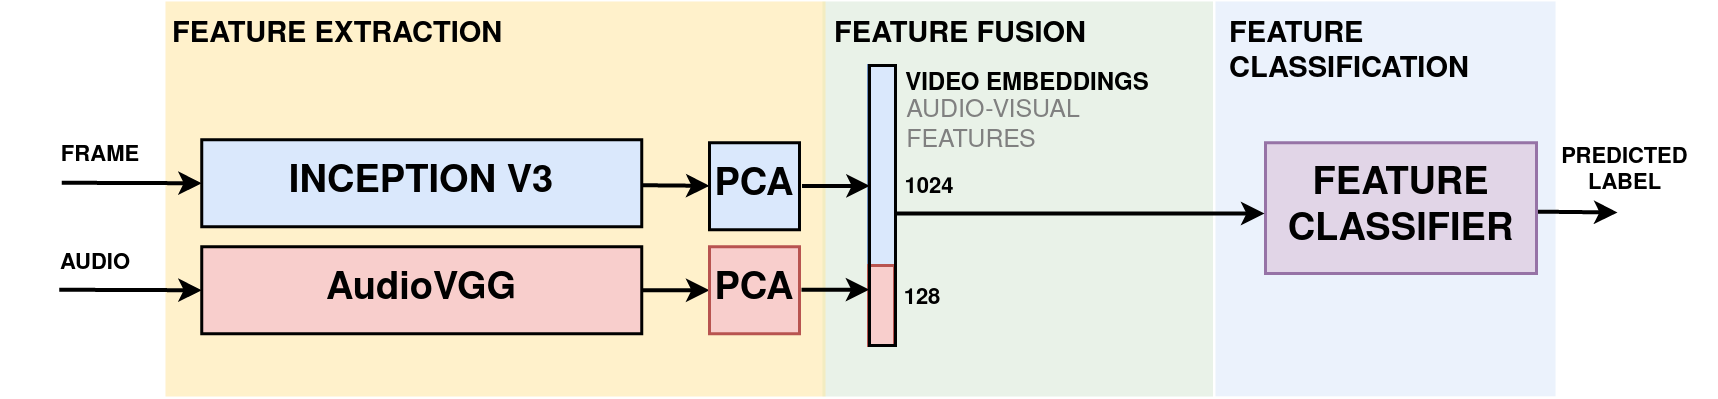
\includegraphics[width=0.9\textwidth]{img/model-2.png}
    \caption{Bimodal architecture for NSFW video classification.}
    \label{fig:model}
    \vspace{-1em}
\end{figure*}

In the feature extraction stage, firstly we split the frames and audio from the video; then, for each media, we use a CNN to extract the features (or embeddings) from each simultaneous video segment. In the second stage, Feature Fusion, we concatenate both audio and frame features. If the classification model is not sequential, we also aggregate the features in this stage. Finally, in the feature classification stage we feed one of the classification models to be experimented with.

\section{Video Embeddings Extraction}
\label{sec:video_features}

CNNs tend to learn low-level features (\textit{e.g.}, in the visual domain: edges, corners, contours) at their first layers. At the intermediate and final layers, the combination of these features helps to extract more complex features, resulting in a vector of continuous values, referred to as \textit{embeddings}, that might be used for classification and other tasks. In this work, we use two benchmark CNNs to extract both image and audio \textit{embeddings} by using a transfer learning technique~\cite{tan2018survey}.


%Afterwards, we apply PCA (+ whitening) to reduce feature dimensions to 1024, followed by quantization (1 byte per coefficient).
%These two compression techniques reduce the size of the data by a factor of 8. The mean vector and covariance matrix for PCA was computed on all frames from the Train partition. We quantize each 32-bit float into 256 distinct values (8 bits) using optimally computed (non-uniform) quantization bin boundaries. We confirmed that the size reduction does not significantly hurt the evaluation metrics. In fact, training all baselines on the full-size data (8 times larger than what we publish), increases all evaluation metrics by less than 1%.
\pva{Falar do pca e da quantizacao?}

By using the feature extraction method created for the Youtube-8m benchmark, we can test an feature extraction method that is powerful enough to represent features that can be in multiple tasks, such as multi-label video classification, video recommendation, and human activity recognition.

"Since the video-level representations are unsupervised (extracted independently of the labels), these representations are far less specialized to the labels associated with the current dataset, and can generalize better to new tasks or video domains."~\cite{abu2016youtube}

In order to validate our dataset, we used the same feature extraction method used in the Youtube-8m dataset challenges~\cite{abu2016youtube}, both networks were pre-trained and frozen. They were not retrained for application sensitive content classification. Which gives future works an opportunity to develop even more efficient and smaller feature extraction networks for this specific task.


As described in ~\cite{abu2016youtube},
To generate image frame features and audio features we decode each video at approximately 1 frame-per-second. For the image frame features, we used an InceptionV3  network~\cite{szegedy2016rethinking} pre-trained on the ImageNet\footnote{\url{http://www.image-net.org/}} dataset. We also use of a AudioVGG~\cite{hershey2017cnn} network with pre-trained weights in the Audioset\footnote{\url{https://research.google.com/audioset/}} dataset to extract the audio embeddings.

Each of these CNNs were used as published by their authors; the only modification was the removal of classification layers in both CNNs to obtain their respective embeddings.

\section{Feature Fusion}
\label{sec:feature_fusion}

Once we have the features from both image and audio, we should make a decision about which method is best to fuse the information from these different domains. Snoek et al. \cite{snoek2005featurefusion} presents two main strategies for information fusion in semantic video analysis: \emph{Early fusion} methods, which works directly with the extracted features, and \emph{Late fusion} methods, which operates on classification outputs from specialized models.
%\pva{For a more recent survey about data fusion and multimedia retrieval, please refer to \cite{jiang2013features}.}
In this work, because we have high abstraction level features, we opted to investigate the most simple approach, which is to use a single model on the concatenated features from both media inputs.

Because of this, in order to create the final embeddings, we concatenate both image and audio embeddings extracted in the same frame and audio window. This generates a sequence of the same size of the number of seconds of the video. After this concatenation, each time-step has 1,152 features: 128 audio features and 1024 frame features.

Notice that with this approach, the video is transformed into a time series, and to use it in non-sequential models (\textit{e.g.}~SVM, KNN, and MLP) we need to turn this sequence into a single feature vector that represents the whole video. In our setting, we did that by taking the average, median, standard deviation, min, and max values for each feature to represent the entire video. In summary, we turn the sequence of features with size $n$ and shape $n$ by 1,152 into a single feature with shape 1 by 5,760.

\section{Classifiers}
\label{sec:classifiers}

% \pva[inline]{porque foi escolhidos esses modelos de classficação, qual a relação deles com o nosso tipo de dado de vídeo.}

For the feature classification task, we will investigate both sequential models (which use the extracted embeddings in a time series format), and non-sequential ones (which use a single aggregated embeddings vector).
We want to experiment with both approaches in order to investigate if a more compact format, such as the single embeddings vector, can yield results at least as good (or even better) than the full feature sequence data.
%Furthermore, we can test if a sequential model can outperform a non-sequential model in specific cases that demand long term memory, such as long videos with very small sensitive scenes.
As an example, one can think of a long video that has a pornographic scene in one second out of its entirety. 
In a non-sequential representation of the extracted features, this short pornographic fragment could be left ``hidden'' among the other non-pornographic frames of the video, as illustrated in Figure \ref{fig:model-non-sequence}.
\begin{figure*}[!ht]
    \centering
    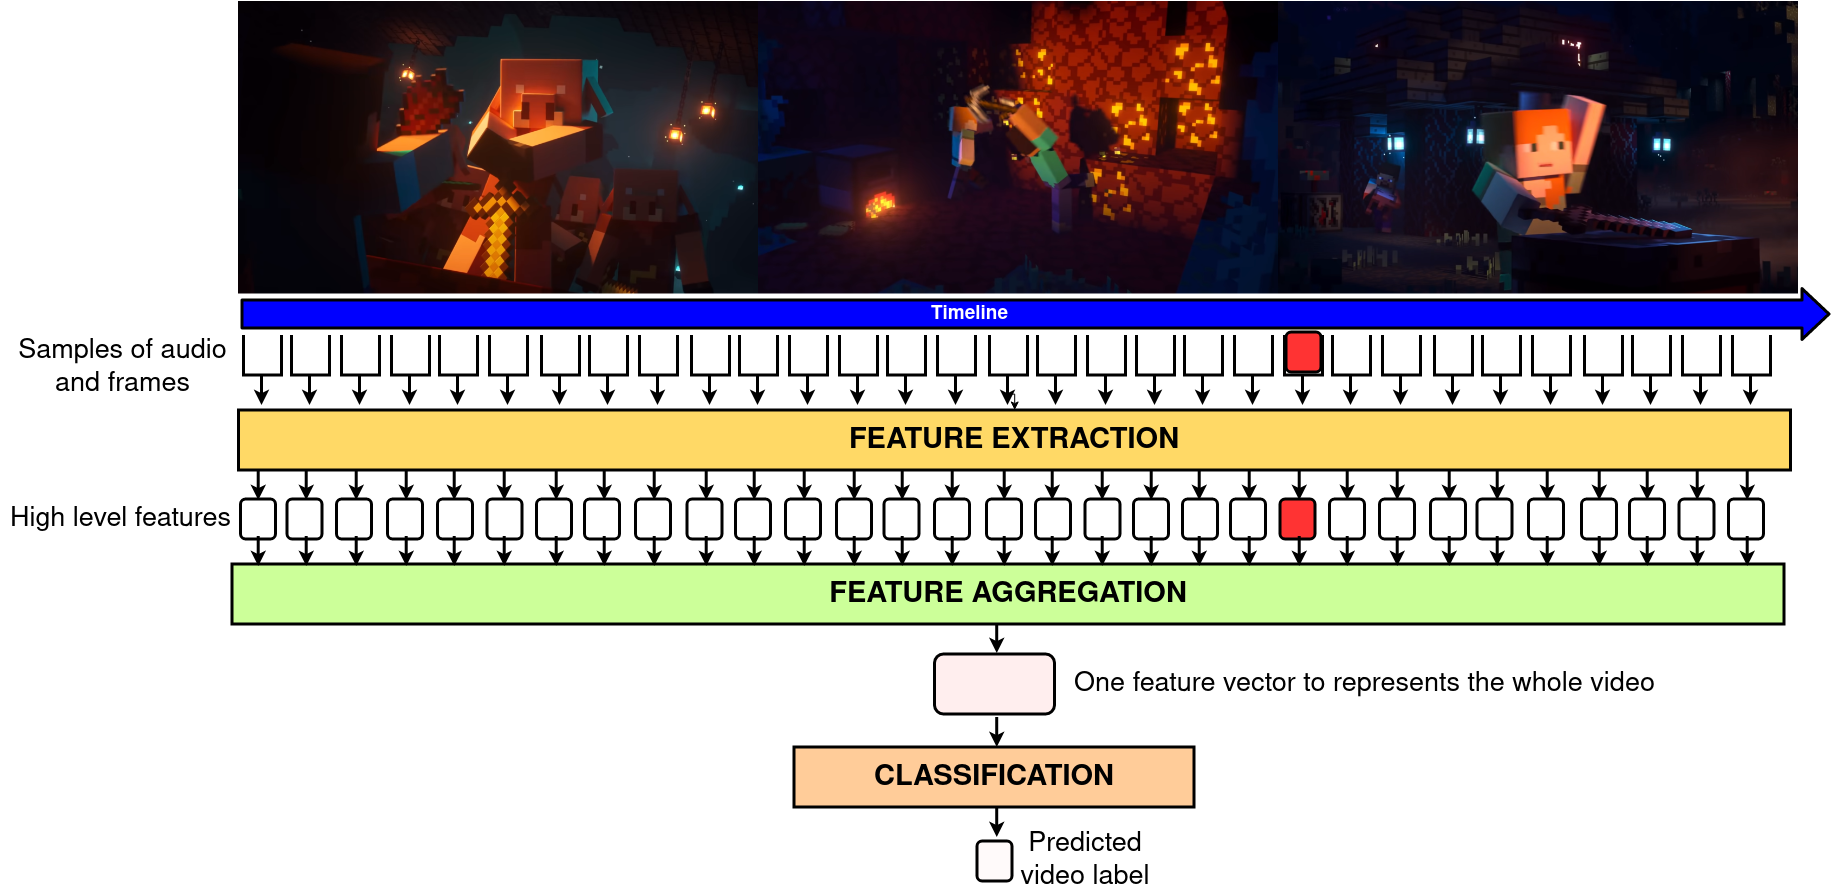
\includegraphics[width=0.9\textwidth]{img/model-non-sequence.png}
    \caption{Sequential features with aggregation, the sensitive scene (red) might vanish among the the other scenes during aggregation.}
    \label{fig:model-non-sequence}
    \vspace{-1em}
\end{figure*}
In a sequential representation, although time series classifiers usually output a prediction after reading the entire sequence, the embedding vectors of each second of the video would not be aggregated and thus could be analysed section by section, as illustrated in Figure \ref{fig:model-sequence}.

\begin{figure*}[!ht]
    \centering
    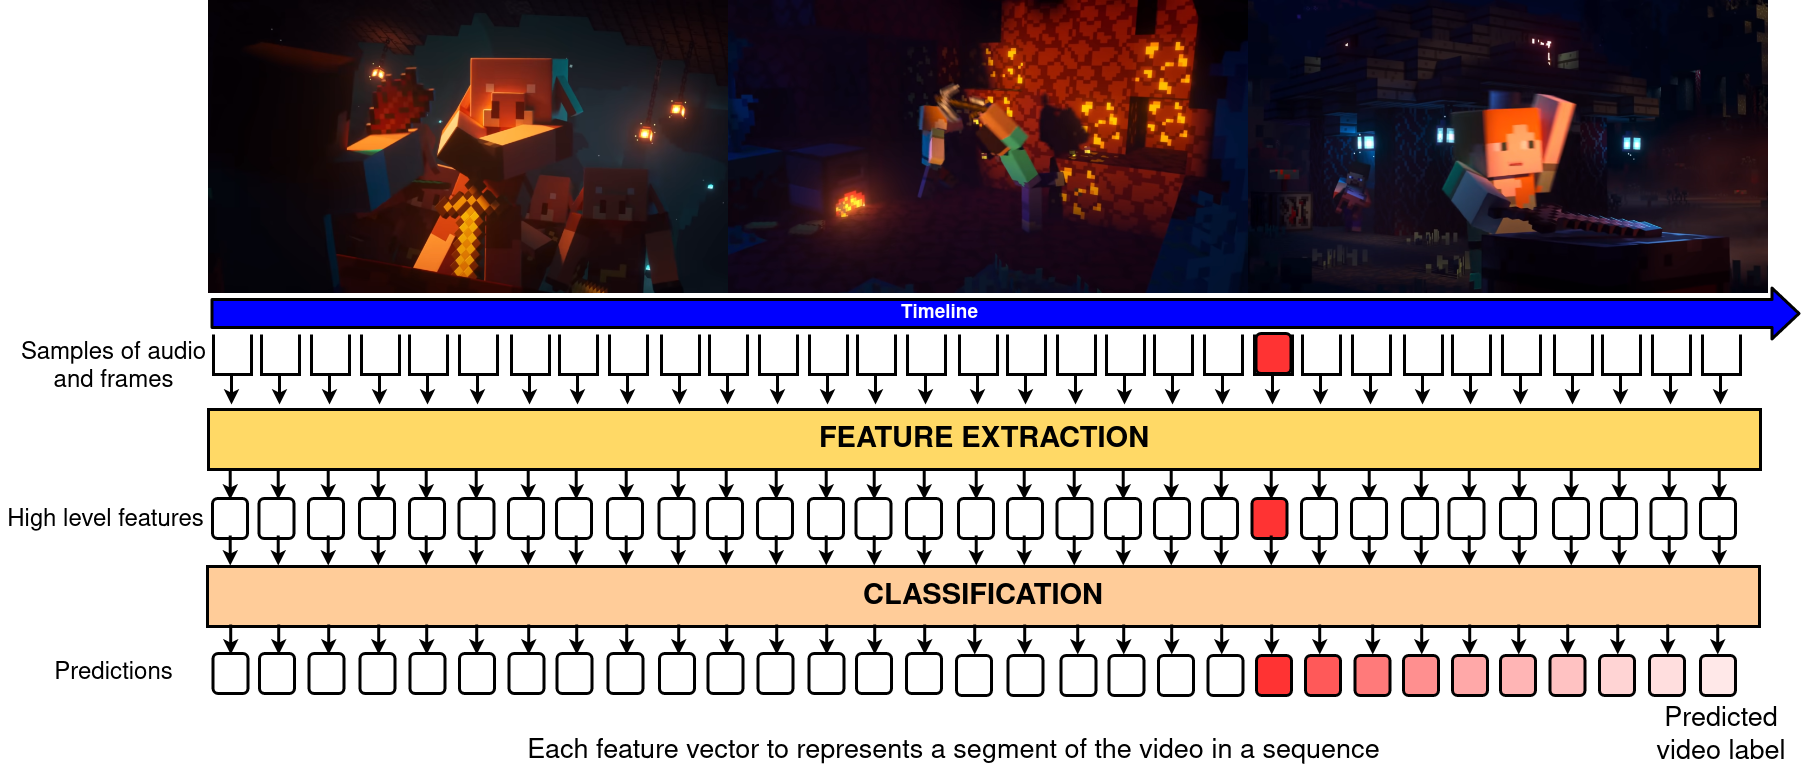
\includegraphics[width=0.9\textwidth]{img/model-sequence.png}
    \caption{Sequential features with no aggregation. In a output after reading the entire sequence, this can also be susceptible to information vanishing.}
    \label{fig:model-sequence}
    \vspace{-1em}
\end{figure*}
Although a sequential representation contains possibly much more redundant data than the non-sequential one, it could give the sequential classification model an important edge of detail over the less granular non-sequential ones.
% To do the feature classification task, we experimented four well known classification mohave dels, one using extracted video features in the time series format, and three that use a single aggregated feature vector.

For the sequential classification model, we chose the Long Short-Term Memory (LSTM)\cite{hochreiter1997long} networks.
It has been a commonly used time series classification baseline model. %\pva{mayber say we'll test GRUs?}

For the non-sequence models, we chose Support Vector Machines (SVM)~\cite{cortes1995support}, K-Nearest Neighbors (KNN)~\cite{peterson2009k}, and Multilayer Perceptron (MLP)~\cite{haykin2009neural}.
Among all of the experimented models, the \textit{Support Vector Machine (SVM)} is the most used in the literature.
% \begin{enumerate}[leftmargin=*]
% \item 
It is a classification model in which the data is mapped into a higher dimension input space, where an optimal separating hyper-plane is constructed.
% These decision surfaces are found by solving a linearly constrained quadratic programming problem.
% \item 
The second model, \textit{K-Nearest Neighbors (KNN)} uses distance measure between training samples so that the k-nearest neighbors always belong to the same class, while samples from different classes are separated by a large margin. 
It was chosen because it used also by related work, although it is a simple classification method.
% \item 
The third model is the \textit{Multilayer-perceptron (MLP)}, which contains layers of nodes: an input layer, an output layer and various hidden layers in between. 
This one was selected because it is also commonly used as a final classifier on deep neural networks.  
% The number of layers used is problem dependent, as is the number of nodes in each hidden layer.
% The weights are adjusted by local optimization using a set of feature vectors so that the network produces the optimal expected output.
% \item 
%Lastly, \textit{Long short-term memory (LSTM)}, different than the feed-forward neural networks, process the entire sequences of data using feedback connections.
% \end{enumerate}
For model evaluation, we performed 20-fold cross validation for all baseline models.
%
\section{Proposed Analysis}\label{sec:experiments}

We evaluate the performances of baseline classifiers over the video \textit{embeddings} that were extracted from our dataset, described in Chapter \ref{chap:dataset}. Then, we choose the best performing classifier during validation stage and test its performance on the \textit{test sets}.  
%\pva{maybe add a image for the process?}
We designed a set of cases that might help us find insights and assess the performance and shortcomings of our dataset and approach.  

% In this work our goal is to create and validate a approach for sensitive content detection in video.

% Some of the questions we aim to answer with this work are:
% \begin{enumerate}
%     \item How does this approach compares with the related work?
%     \item What is the impact of also using audio in the model's performance?
%     \item Can the same model have a performance higher than 90\% on both pornography and violence detection tasks?
% \end{enumerate}

Our objective with these analysis is to attest the quality of our dataset and approach at detecting sensitive content on video.

We did not perform extensive hiperparameter optimization on the baseline models, we performed most hiperparameters changes on the SVM model, since it is the model most sensitive to hiperparameters optimization.
%, while also answering our research questions, stated in Section \ref{sec:introduction}.
% In this analysis, our objective is to attest to the quality of our video \textit{embeddings}.
 
% In the next subsections, we discuss the analysis setup, used metrics, and our findings. In Subsection \ref{sec:config} we describe the training configuration for each model.
% Next, in Subsection \ref{sec:metrics} we describe the evaluation metrics.
% And finally, in Subsection \ref{sec:results} we present our empirical findings.
\begin{enumerate}[start=0,label={(\bfseries E\arabic*):}]
%\item The sensitive content detection task: This is the main analysis of this work, in this analysis we test the capabilities of our approach and the best performing classification model on our test subset.%\pva{maybe referenciar ao subset de teste do nosso dataset?}

%\item The pornography detection task: In this analysis we evaluate our approach and the best performing classification model on the pornography detection task using our test subset. 

%\item The gore detection task: In this analysis we evaluate our approach and the best performing classification model on the gore detection task using our test subset.

\item Testing only on image features: In this analysis we evaluate our approach on the our test subset using the visual (frames) features only.

\item Testing only on audio features: In this analysis we evaluate our approach on the our test subset using the audio features only.

%\item Testing on the pornography-2k: In this analysis we evaluate our approach on the pornography-2k dataset.

\item Testing pornography using audio only videos: In this analysis we evaluate our approach on the pornography-2k dataset using the audio features only.

\item Testing pornography using only on image features: In this analysis we evaluate our approach on the pornography-2k dataset using the visual features only.
%\item esting MEDIAEVAL Violent Scenes Dataset

\item Investigate misclassified videos in the test sets: In this analysis case we search for insights on what videos our approach fails to correctly detect sensitive content.
% \item sequence classification models vs non-sequence models
\end{enumerate}

In the next Chapter, we present and discuss the results of our baselines and report each analysis.